%% For double-blind review submission, w/o CCS and ACM Reference (max submission space)
\documentclass[sigplan,review,anonymous]{acmart}\settopmatter{printfolios=true,printccs=false,printacmref=false}
%% For double-blind review submission, w/ CCS and ACM Reference
%\documentclass[sigplan,review,anonymous]{acmart}\settopmatter{printfolios=true}
%% For single-blind review submission, w/o CCS and ACM Reference (max submission space)
%\documentclass[sigplan,review]{acmart}\settopmatter{printfolios=true,printccs=false,printacmref=false}
%% For single-blind review submission, w/ CCS and ACM Reference
%\documentclass[sigplan,review]{acmart}\settopmatter{printfolios=true}
%% For final camera-ready submission, w/ required CCS and ACM Reference
%\documentclass[sigplan]{acmart}\settopmatter{}


%% Conference information
%% Supplied to authors by publisher for camera-ready submission;
%% use defaults for review submission.
\acmConference[PL'18]{ACM SIGPLAN Conference on Programming Languages}{January 01--03, 2018}{New York, NY, USA}
\acmYear{2018}
\acmISBN{} % \acmISBN{978-x-xxxx-xxxx-x/YY/MM}
\acmDOI{} % \acmDOI{10.1145/nnnnnnn.nnnnnnn}
\startPage{1}

%% Copyright information
%% Supplied to authors (based on authors' rights management selection;
%% see authors.acm.org) by publisher for camera-ready submission;
%% use 'none' for review submission.
\setcopyright{none}
%\setcopyright{acmcopyright}
%\setcopyright{acmlicensed}
%\setcopyright{rightsretained}
%\copyrightyear{2018}           %% If different from \acmYear

%% Bibliography style
\bibliographystyle{ACM-Reference-Format}
%% Citation style
%\citestyle{acmauthoryear}  %% For author/year citations
%\citestyle{acmnumeric}     %% For numeric citations
%\setcitestyle{nosort}      %% With 'acmnumeric', to disable automatic
                            %% sorting of references within a single citation;
                            %% e.g., \cite{Smith99,Carpenter05,Baker12}
                            %% rendered as [14,5,2] rather than [2,5,14].
%\setcitesyle{nocompress}   %% With 'acmnumeric', to disable automatic
                            %% compression of sequential references within a
                            %% single citation;
                            %% e.g., \cite{Baker12,Baker14,Baker16}
                            %% rendered as [2,3,4] rather than [2-4].

%!TEX root = main.tex

\newcommand{\set}[1]{\{ #1 \}}
\newcommand{\sequence}[2]{(#1, \ldots, #2)}
\newcommand{\couple}[2]{(#1,#2)}
\newcommand{\pair}[2]{(#1,#2)}
\newcommand{\triple}[3]{(#1,#2,#3)}
\newcommand{\quadruple}[4]{(#1,#2,#3,#4)}
\newcommand{\tuple}[2]{(#1,\ldots,#2)}
\newcommand{\Nat}{\ensuremath{\mathbb{N}}}
\newcommand{\Rat}{\ensuremath{\mathbb{Q}}}
\newcommand{\Rea}{\ensuremath{\mathbb{R}}}
\newcommand{\Int}{\ensuremath{\mathbb{Z}}}
%\newcommand{\true}{\top}
%\newcommand{\false}{\perp}
\newcommand{\bottom}{\perp}
%% \newcommand{\powerset}[1]{{\cal P}(#1)}
\newcommand{\npowerset}[2]{{\cal P}^{#1}(#2)}
\newcommand{\finitepowerset}[1]{{\cal P}_f(#1)}
\newcommand{\level}[2]{L_{#1}(#2)}
\newcommand{\card}[1]{\mbox{card}(#1)}
\newcommand{\range}[1]{\mathtt{ran}(#1)}
\newcommand{\astring}{s}

\newcommand{\Cc}{\mathcal{C}}

\newcommand{\intnum}{\mathbb{Z}}


\newcommand {\notof}{\ensuremath{\neg}}
\newcommand {\myand}{\ensuremath{\wedge}}
\newcommand {\myor}{\ensuremath{\vee}}
\newcommand {\mynext}{\mbox{{\sf X}}}
\newcommand {\until}{\mbox{{\sf U}}}
\newcommand {\sometimes}{\mbox{{\sf F}}}
\newcommand {\previous}{\mynext^{-1}}
\newcommand {\since}{\mbox{{\sf S}}}
\newcommand {\fminusone}{\mbox{{\sf F}}^{-1}}
\newcommand {\everywhere}[1]{\mbox{{\sf Everywhere}}(#1)}



\newcommand{\aatomic}{{\rm A}}
\newcommand{\aset}{X}
\newcommand{\asetbis}{Y}
\newcommand{\asetter}{Z}

\newcommand{\avarprop}{p}
\newcommand{\avarpropbis}{q}
\newcommand{\avarpropter}{r}
\newcommand{\varprop}{{\rm PROP}} % Set of atomic propositions (for a given logic)

% formulae

\newcommand{\aformula}{\astateformula} % a formula
\newcommand{\aformulabis}{\astateformulabis} % another formula (when at least 2 are present)
\newcommand{\aformulater}{\astateformulater} % another formula (when at least 3 are present)
\newcommand{\asetformulae}{X}
\newcommand{\subf}[1]{sub(#1)}

\newcommand{\aautomaton}{{\mathbb A}}
\newcommand{\aautomatonbis}{{\mathbb B}}

%\newcommand {\length}[1] {\ensuremath{|#1|}}



% Equivalences
\newcommand{\egdef}{\stackrel{\mbox{\begin{tiny}def\end{tiny}}}{=}} % =def=
\newcommand{\eqdef}{\stackrel{\mbox{\begin{tiny}def\end{tiny}}}{=}} % =def=
\newcommand{\equivdef}{\stackrel{\mbox{\begin{tiny}def\end{tiny}}}{\equivaut}} % <=def=>
\newcommand{\equivaut}{\;\Leftrightarrow\;}

\newcommand{\ainfword}{\sigma}

\newcommand{\amap}{\mathfrak{f}}
\newcommand{\amapbis}{\mathfrak{g}}

\newcommand{\step}[1]{\xrightarrow{\!\!#1\!\!}}
\newcommand{\backstep}[1]{\xleftarrow{\!\!#1\!\!}}

\newcommand {\aedge}[1] {\ensuremath{\stackrel{#1}{\longrightarrow}}}
\newcommand {\aedgeprime}[1] {\ensuremath{\stackrel{#1}{\longrightarrow'}}}
\newcommand {\afrac}[1] {\ensuremath{\mathit{frac}(#1)}}
\newcommand {\cl}[1] {\ensuremath{\mathit{cl}(#1)}}
\newcommand {\sfc}[1] {\ensuremath{\mathit{sfc}(#1)}}
\newcommand {\dunion} {\ensuremath{\uplus}}
\newcommand {\edge} {\ensuremath{\longrightarrow}}
\newcommand {\emptyword}{\ensuremath{\epsilon}}
\newcommand {\floor}[1] {\ensuremath{\lfloor #1 \rfloor}}
\newcommand {\intersection} {\ensuremath{\cap}}
\newcommand {\union} {\ensuremath{\cup}}
\newcommand {\vals}[2] {\ensuremath{\mathit{val}_{#2}(#1)}}



\newcommand {\pspace} {\textsc{pspace}}
\newcommand {\nlogspace} {\textsc{nlogspace}}
\newcommand {\logspace} {\textsc{logspace}}
\newcommand {\expspace} {\textsc{expspace}}
\newcommand {\nexpspace} {\textsc{nexpspace}}
\newcommand {\exptime} {\textsc{exptime}}
\newcommand {\np} {\textsc{np}}
\newcommand {\threeexptime} {\textsc{3exptime}}
\newcommand {\polytime} {\textsc{p}}
\newcommand{\twoexpspace}{\textsc{2expspace}}
\newcommand{\threeexpspace}{\textsc{3expspace}}
\newcommand {\nexptime} {\textsc{nexptime}}

\newcommand {\nonelementary} {\textsc{non-elementary}}

\newcommand {\elementary} {\textsc{elementary}}


\newcommand{\aalphabet}{\Sigma}     % an alphabet, A is already used for atoms
\newcommand{\aword}{\mathfrak{u}}
\newcommand{\awordbis}{\mathfrak{v}}



\newcommand{\aassertion}{P}
\newcommand{\aassertionbis}{Q}
\newcommand{\aexpression}{e}
\newcommand{\aexpressionbis}{f}
\newcommand{\avariable}{\mathtt{x}}
\newcommand{\uniquevar}{\mathtt{u}}
\newcommand{\uniquevarbis}{\mathtt{v}}
\newcommand{\avariablebis}{\mathtt{y}}
\newcommand{\avariableter}{\mathtt{z}}
\newcommand{\nullconstant}{\mathtt{null}}
\newcommand{\nilvalue}{nil}
\newcommand{\emptyconstant}{\mathtt{emp}}
\newcommand{\infheap}{\mathtt{inf}}
\newcommand{\saturated}{\mathtt{Saturated}}

\newcommand{\astateformula}{\phi}
\newcommand{\astateformulabis}{\psi}
\newcommand{\astateformulater}{\varphi}
%%
\newcommand{\separate}{\ast}
\newcommand{\sep}{\separate}
\newcommand{\size}{\mathtt{size}}
\newcommand{\sizeeq}[1]{\mathtt{size} \ = \ #1}
\newcommand{\alloc}[1]{\mathtt{alloc}(#1)}
\newcommand{\allocb}[2]{\mathtt{alloc}^{-1}[#2](#1)}
\newcommand{\isol}[1]{\mathtt{isoloc}(#1)}
\newcommand{\icell}{\mathtt{isocell}}
\newcommand{\malloc}{\mathtt{malloc}}
\newcommand{\cons}{\mathtt{cons}}
\newcommand{\new}{\mathtt{new}}
\newcommand{\free}[1]{\mathtt{free} \ #1}
\newcommand{\maxform}[1]{\mathtt{maxForms}(#1)}
\newcommand{\locations}[1]{\mathtt{loc}(#1)}
\newcommand{\values}{\mathtt{Val}}
\newcommand{\aheap}{\mathfrak{h}}
\newcommand{\avaluation}{\mathfrak{V}}
\newcommand{\heaps}{\mathcal{H}}
\newcommand{\astore}{\mathfrak{s}}
\newcommand{\stores}{\mathcal{S}}
\newcommand{\amodel}{\mathfrak{M}}
\newcommand{\alabel}{\ell}

\newcommand{\aprogram}{\mathtt{PROG}}
\newcommand{\programs}{\mathtt{P}}
\newcommand{\ctprograms}{\programs^{ct}}
\newcommand{\aninstruction}{\mathtt{instr}}
\newcommand{\ainstruction}{\mathtt{instr}}
\newcommand{\instructions}{\mathtt{I}}
\newcommand{\aguard}{\ensuremath{g}}
\newcommand{\guards}{\ensuremath{G}}
\newcommand{\domain}[1]{\mathtt{dom}(#1)}
\newcommand{\memory}{\stores\times\heaps}
\newcommand{\skipinstruction}{\mathtt{skip}}

\newcommand{\execution}{\mathtt{comp}}
\newcommand{\aux}{\mathtt{embd}}
\newcommand{\runof}{run}
\newcommand{\anexecution}{e}


\newcommand{\aletter}{\ensuremath{a}}
\newcommand{\aletterbis}{\ensuremath{b}}
\newcommand{\alocation}{\mathfrak{l}}

\newcommand{\pointsl}[1]{\stackrel{#1}{\hookrightarrow}}
\newcommand{\ppointsl}[1]{\stackrel{#1}{\mapsto}}
\newcommand{\ourhook}[1]{\stackrel{#1}{\hookrightarrow}}
\newcommand{\ltrue}{{\sf true}}
\newcommand{\lfalse}{{\sf false}}


\newcommand{\variables}{\mathtt{FVAR}}
\newcommand{\pvariables}{\mathtt{PVAR}}
\newcommand{\secvariables}{\mathtt{SVAR}}
\newcommand{\logique}[1]{\mathtt{FO}(#1)}



\newcommand{\atranslation}{\mathfrak{t}}
\newcommand{\nbpred}[1]{\widetilde{\sharp #1}}
\newcommand{\nbpredstar}[1]{\widetilde{\sharp #1}^{\star}}
\newcommand{\isolated}{\mathtt{isol}}
\newcommand{\stdmarks}{\mathtt{envir}}
\newcommand{\relation}[1]{\mathtt{relation}_{#1}}
\newcommand{\freevar}{\mathtt{FV}}
\newcommand{\notonmark}{\mathtt{notonenv}}
\newcommand{\InVal}[1]{\mathtt{InVal}\!\left(#1\right)}
\newcommand{\NotOnEnv}[1]{\mathtt{NotOnEnv}\!\left(#1\right)}
\newcommand{\PartOfVal}[1]{\mathtt{PartOfVal}\!\left(#1\right)}
%\newcommand{\nbpreds}[3]{\sharp #1 \geq #2}
\newcommand{\defstyle}[1]{{\emph{#1}}}

\newcommand{\cut}[1]{}
\newcommand{\interval}[2]{[#1,#2]}
\newcommand{\buniquevar}{\overline{\uniquevar}}
\newcommand{\bbuniquevar}{\overline{\overline{\uniquevar}}}
\newcommand{\magicwand}{\mathop{\mbox{$\mbox{$-~$}\!\!\!\!\ast$}}}
\newcommand{\wand}{\magicwand}
\newcommand{\septraction}{\stackrel{\hsize0pt \vbox to0pt{\vss\hbox to0pt{\hss\raisebox{-6pt}{\footnotesize$\lnot$}\hss}\vss}}{\magicwand}}
%% \newcommand{\reach}{\mathtt{reach}}
\mathchardef\mhyphen="2D % hyphen while in math mode

\newcommand{\adataword}{\mathfrak{dw}}
\newcommand{\adatum}{\mathfrak{d}}

\newcommand{\collectionknives}{\mathtt{ks}}
\newcommand{\collectionknivesfork}[1]{\mathtt{ksfs}_{=#1}}
\newcommand{\collectionknivesforks}{\mathtt{ksfs}}
\newcommand{\collectionkniveslargeforks}{\mathtt{kslfs}}


\newcommand{\acounter}{\mathtt{C}}

\newcommand{\fotwo}[3]{{\mbox{FO2}_{#1,#2}(#3)}}
\newcommand{\mtrans}[1]{t\!\left(#1\right)^{\Box}}
\newcommand{\mbtrans}[2]{\mtrans{#2}_{#1}}


\newcommand{\alogic}{\mathfrak{L}}


\newcommand{\semantics}[1]{\ensuremath{[ #1 ]}}


\newcommand{\adomino}{\mathfrak{d}}
\newcommand{\atile}{\mathfrak{d}}
\newcommand{\atiling}{\mathfrak{t}}

\newcommand{\hori}{\mathtt{h}}
\newcommand{\verti}{\mathtt{v}}
\newcommand{\domi}{\mathtt{d}}

\newcommand{\cpyrel}{\mathfrak{cp}}

\newcommand{\cntcmp}{\mathfrak{C}}

\newcommand{\heapdag}{\mathfrak{G}}

\newcommand{\onmainpath}{\mathtt{mp}}

\newcommand{\tree}{\mathtt{tree}}

%\newcommand{\tile}{\mathtt{tile}}

\newcommand{\type}{\mathtt{type}}

\newcommand{\ptype}{\mathtt{ptype}}

\newcommand{\exttype}{\mathtt{exttype}}

\newcommand{\anctypes}{\mathtt{AncTypes}}

\newcommand{\destypes}{\mathtt{DesTypes}}

\newcommand{\inctypes}{\mathtt{IncTypes}}

\newcommand{\treeic}{\mathtt{treeIC}}

\newcommand{\trs}{\mathfrak{trs}}


\newcommand{\nin}{\not \in}
\newcommand{\cupplus}{\uplus}
\newcommand{\aunarypred}{\mathtt{P}}


\newcommand{\hide}[1]{}

\newcommand{\eval}[2]{\llbracket#1\rrbracket_{#2}}
\newcommand\cur{\mathsf{cur}}
\newcommand\dom{\mathsf{dom}}
\newcommand\rng{\mathsf{rng}}

\newcommand\dd{\mathbb{D}}
\newcommand\nat{\mathbb{N}}


\newcommand\cA{\mathcal{A}}
\newcommand\cB{\mathcal{B}}
\newcommand\cC{\mathcal{C}}
\newcommand\cE{\mathcal{E}}
\newcommand\cG{\mathcal{G}}
\newcommand\Ll{\mathcal{L}}
\newcommand\cM{\mathscr{M}}
\newcommand\cP{\mathcal{P}}
\newcommand\cR{\mathcal{R}}
\newcommand\cS{\mathcal{S}}
\newcommand\cT{\mathcal{T}}

\newcommand\vard{\mathfrak{d}}

\newcommand\replace{\mathsf{replace}}
\newcommand\replaceall{\mathsf{replaceAll}}
\newcommand\sreplaceall{\mathsf{sreplaceAll}}
\newcommand\reverse{\mathsf{reverse}}
\newcommand\indexof{\mathsf{indexOf}}
\newcommand\length{\mathsf{length}}
\newcommand\substring{\mathsf{substring}}
\newcommand\charat{\mathsf{charAt}}
\newcommand\extract{\mathsf{extract}}

\newcommand\revsym{\pi}

\newcommand\strline{\mathsf{SL}}

\newcommand\pstrline{\mathsf{SL_{pure}}}

\newcommand\search{\mathsf{search}}

\newcommand\verify{\mathsf{vfy}}

\newcommand\searchleft{\mathsf{left}}

\newcommand\searchlong{\mathsf{long}}


\newcommand\pref{\mathsf{Pref}}

\newcommand\wprof{\mathsf{WP}}

\newcommand\vars{\mathsf{Vars}}

\newcommand\dep{\mathsf{Dep}}
\newcommand\ptn{\mathsf{Ptn}}

\newcommand\src{\mathsf{src}}
\newcommand\strtorep{\mathsf{strToRep}}

\newcommand\rpleft{\mathsf{l}}
\newcommand\rpright{\mathsf{r}}


\newcommand\srcnd{\mathsf{srcND}}

\newcommand\ctxt{\mathsf{ctxt}}


\newcommand\ctxts{\mathsf{Ctxts}}

\newcommand\sprt{\mathsf{sprt}}

\newcommand\val{\mathsf{val}}

\newcommand\srclen{\mathsf{srcLen}}

\newcommand\rpleftlen{\mathsf{lLen}}


\newcommand\dfs{\mathsf{DFS}}

\newcommand\repr{\mathsf{rep}}

\newcommand\red{\mathsf{red}}

\newcommand\gfun{\mathcal{F}}


\newcommand{\leftmost}{{\sf leftmost}}
\newcommand{\longest}{{\sf longest}}

\newcommand{\arbidx}{{\sf Idx_{arb}}}
\newcommand{\dmdidx}{{\sf Idx_{dmd}}}
\newcommand{\lftlen}{{\sf Len_{lft}}}


\newcommand{\ASSERT}[1]{\textsf{assert}\left(#1\right)}

\newcommand{\concat}{\cdot}

\newcommand{\parabs}{\Theta} % parametr abstraction
\newcommand{\arity}{r}

\newcommand{\FA}{FA}
\newcommand{\FFA}{2FA}
\newcommand{\SFFA}{S2FA}
\newcommand{\FT}{FT}
\newcommand{\FFT}{2FT}
\newcommand{\FunFT}{FFT}
\newcommand{\SFFT}{S2FT}
\newcommand{\PT}{PT}
\newcommand{\PPT}{2PT}
\newcommand{\SPPT}{S2PT}
\newcommand{\RBPPT}{RB2PT}
\newcommand{\RBSPPT}{RBS2PT}
\newcommand{\SA}{SA}
\newcommand{\SSA}{2SA}
\newcommand{\ST}{ST}
\newcommand{\SST}{2ST}
\newcommand{\SPT}{SPT}
\newcommand{\SSPT}{2SPT}
\newcommand{\RBSSPT}{RB2SPT}

\newcommand{\ialphabet}{\Sigma}
\newcommand{\oalphabet}{\Gamma}


\newcommand{\EndLeft}{\ensuremath{\vartriangleright}}
\newcommand{\EndRight}{\ensuremath{\vartriangleleft}}

\newcommand{\Lang}{\mathscr{L}}
\newcommand{\Tran}{\mathscr{T}}

\newcommand{\NFA}{\mathcal{A}}
\newcommand{\NFAB}{\mathcal{B}}
\newcommand{\NFT}{\mathcal{T}}

\newcommand{\CEFA}{\mathcal{A}}

\newcommand{\Transducer}{\ensuremath{T}}
\newcommand{\controls}{\ensuremath{Q}}
\newcommand{\finals}{\ensuremath{F}}
\newcommand{\transrel}{\ensuremath{\delta}}


\newcommand{\Left}{\ensuremath{-1}}
\newcommand{\Right}{\ensuremath{1}}
\newcommand{\Stay}{\ensuremath{0}}


\newcommand{\defn}[1]{\emph{#1}}

\newcommand{\conacc}{\Omega}

\newcommand{\reginvrel}{\textbf{RegInvRel}}

\newcommand{\prerec}{\reginvrel}

\newcommand{\regmondec}{\textbf{RegMonDec}}

\newcommand\rcdim{\mathsf{art}}

\newcommand\rcdep{\mathsf{asgn}}

\newcommand\rcasrt{\mathsf{asrt}}

\newcommand\rcreg{\mathsf{reg}}

\newcommand\rcsreg{\mathsf{sreg}}


\newcommand\tower{\mathrm{Tower}}

\newcommand\rcphi{\mathsf{fnsize}}
\newcommand\rcpsi{\mathsf{fasize}}

%%%%%%%%%%%%
% Auto escape eg

\newcommand\linkvar{\mintinline{html}{$li}}
\newcommand\linktextvar{\mintinline{html}{$txt}}
\newcommand\urlstarttag{\texttt{[URL]}}
\newcommand\urlendtag{\texttt{[LRU]}}
\newcommand\htmlstarttag{\texttt{[HTML]}}
\newcommand\htmlendtag{\texttt{[LMTH]}}

\newcommand{\Pre}{\textsf{Pre}}

\newcommand\bigO{\mathcal{O}}

\newcommand\Aut{\mathcal{A}}

\newcommand{\tup}[1]{\left( #1 \right)}

\newcommand\ap[2]{{#1}\mathord{\brac{#2}}}
%\newcommand\ap[2]{{#1}\mathord{\brac{#2}}}

\newcommand{\opset}{\mathscr{O}}

\newcommand{\strlineall}{$\strline$[\FT, $\replaceall$, $\reverse$]}

\newcommand{\strlineconcat}{$\strline$[$\concat$, $\sreplaceall$, $\reverse$, \FT]}

\newcommand{\strlinefft}{$\strline$[$\concat$, $\replaceall$, $\reverse$, \FunFT]}


%%% Macros for expspace lower bound with replaceall

% General
\newcommand\brac[1]{\left(#1\right)}

% \setcomp{ele}{comp} = { ele | comp }
\newcommand\setcomp[2]{\left\{{#1}\ \middle|\ {#2}\right\}}

% \lang{A} = L(A)
\newcommand\lang[1]{\mathcal{L}\mathord{\brac{#1}}}

%% Optimisations

\newcommand\caleybox[1]{\llparenthesis #1 \rrparenthesis}
\newcommand\internalchar{\flat}

% Tools

\newcommand\stranger{Stranger}

\newcommand\transducerbench{\textsc{Transducer}}
\newcommand\slogbench{\textsc{SLOG+}}
\newcommand\slogbenchr{\textsc{SLOG+(replace)}}
\newcommand\slogbenchra{\textsc{SLOG+(replaceall)}}
\newcommand\kaluzabench{\textsc{Kaluza}}
\newcommand\pyexbench{\textsc{PyEx}}
\newcommand\pyextdbench{\textsc{PyEx-}td}
\newcommand\pyexztbench{\textsc{PyEx-}z3}
\newcommand\pyexzzbench{\textsc{PyEx-}zz}

\newtheorem{fact}{Fact}
\newtheorem{remark}{Remark}


\newcommand\slint{${\rm SL}_{\rm int}$}

\newcommand\cslint{SL$^{\dag}_{int}$}

\newcommand{\regexp} {{\sf Regex}}
%\newcommand{\cgexp} {{\sf RWRE_{reg}}}
\newcommand{\pcre} {{\sf PCRE}}

\newcommand{\lasat}{${\rm SAT}_{\rm CEFA}[{\rm LIA}]$}

\newcommand{\prjnum}{{\rm Prj}_{\rm num}}

\newcommand{\uwp}{{\rm uwp}}

\newcommand\urlxsssanitise{{\sf urlXssSanitise}}

%%%%%%%%%% Start TeXmacs macros
\newcommand{\colons}{\,:\,}
\newcommand{\tmop}[1]{\ensuremath{\operatorname{#1}}}
\newcommand{\tmtextit}[1]{{\itshape{#1}}}
\newcommand{\tmtextbf}[1]{{\bfseries{#1}}}
%\newtheorem{definition}{Definition}
%{\theorembodyfont{\rmfamily}\newtheorem{note}{Note}}
%{\theorembodyfont{\rmfamily}\newtheorem{remark}{Remark}}
%\newtheorem{theorem}{Theorem}
%\newtheorem{note}{Note}
%\newtheorem{remark}{Remark}
\newcommand\NSST{{\sf NSST}}
\newcommand\PSST{{\sf PSST}}
\newcommand\refexp{{\sf REP}}
\newcommand\ssym{{\sf Start}}
\newcommand\esym{{\sf End}}

\newcommand\pnfa{\mathcal{A}}
\newcommand\psst{\mathcal{T}}

\newcommand\pat{\mathsf{pat}}
\newcommand\rep{\mathsf{rep}}

\newcommand\refbefore{\$^{\leftarrow}}
\newcommand\refafter{\$^{\rightarrow}}

\newcommand\nullchar{\mathsf{null}}

\newcommand\idxexp{{\sf idx}}


\newcommand\cvc{CVC4}
\newcommand\zthree{Z3-str3}
\newcommand\trau{Trau}
\newcommand\trauplus{Trau+}
\newcommand\zthreetrau{Z3-Trau}
\newcommand\ostrich{EMU}
\newcommand\expose{ExpoSE}
\newcommand\sloth{Sloth}
\newcommand\slent{Slent}
\newcommand\Tool{\text{OSTRICH+}}
\newcommand{\OMIT}[1]{}

\newcommand{\seq}[1]{\ensuremath{#1}}
\newcommand{\seqq}[1]{\seq{\Gamma\ifx#1\relax\else,#1\fi}}

\newcommand{\infer}[3][]{%
  \AxiomC{$#3$}
  \ifx#1\relax\else\LeftLabel{\textsc{#1}}\fi
  \UnaryInfC{$#2$}
  \DisplayProof
}
\newcommand{\inferC}[3]{%
  \AxiomC{$#3$}
  \RightLabel{$~~#1$}
  \UnaryInfC{$#2$}
  \DisplayProof
}
\newcommand{\inferii}[4][]{%
  \AxiomC{$#3$}
  \AxiomC{$#4$}
  \ifx#1\relax\else\LeftLabel{\textsc{#1}}\fi
  \BinaryInfC{$#2$}
  \DisplayProof
}


\usepackage{mathrsfs}

\newif\ifdraft\drafttrue
%\newif\ifdraft\draftfalse
\ifdraft
\newcommand{\anthony}[1]{\color{red} {AL: #1 :LA} \color{black}}
\newcommand{\zhilin}[1]{\color{brown} {ZL: #1 :LZ} \color{black}}
\newcommand{\tl}[1]{\color{blue} {TL: #1 :LT} \color{black}}
\newcommand{\mat}[1]{\color{cyan} {MH: #1 :HM} \color{black}}
\newcommand{\philipp}[1]{\color{magenta} {PR: #1 :PR} \color{black}}
\newcommand{\zhilei}[1]{\color{violet} {ZLH: #1 :HZL} \color{black}}
\else
\newcommand{\anthony}[1]{}
\newcommand{\zhilin}[1]{}
\newcommand{\tl}[1]{}
\newcommand{\mat}[1]{}
\newcommand{\zhilei}[1]{}
\fi

%%%%%%%%%% Start TeXmacs macros
\newcommand{\colons}{\,:\,}
\newcommand{\tmop}[1]{\ensuremath{\operatorname{#1}}}
\newcommand{\tmtextit}[1]{{\itshape{#1}}}
\newcommand{\tmtextbf}[1]{{\bfseries{#1}}}
\newtheorem{definition}{Definition}
%{\theorembodyfont{\rmfamily}\newtheorem{note}{Note}}
%{\theorembodyfont{\rmfamily}\newtheorem{remark}{Remark}}
\newtheorem{theorem}{Theorem}
%\newtheorem{note}{Note}
\newtheorem{remark}{Remark}
\newcommand\NSST{{\sf NSST}}
\newcommand\PSST{{\sf PSST}}
\newcommand\refexp{{\sf REF}}
\newcommand\ssym{{\sf Start}}
\newcommand\esym{{\sf End}}

\newcommand\pnfa{\mathcal{N}}
\newcommand\psst{\mathcal{T}}

\newcommand\pat{\mathsf{pat}}
\newcommand\rep{\mathsf{rep}}
%%%%%%%%%% End TeXmacs macros




%%%%%%%%%%%%%%%%%%%%%%%%%%%%%%%%%%%%%%%%%%%%%%%%%%%%%%%%%%%%%%%%%%%%%%
%% Note: Authors migrating a paper from traditional SIGPLAN
%% proceedings format to PACMPL format must update the
%% '\documentclass' and topmatter commands above; see
%% 'acmart-pacmpl-template.tex'.
%%%%%%%%%%%%%%%%%%%%%%%%%%%%%%%%%%%%%%%%%%%%%%%%%%%%%%%%%%%%%%%%%%%%%%



\begin{document}

%% Title information
\title{Solving String Constraints with Practical Regular Expressions}



%% Author with single affiliation.
\author{Taolue Chen}
%\authornote{with author1 note}          %% \authornote is optional;
                                        %% can be repeated if necessary
%\orcid{nnnn-nnnn-nnnn-nnnn}             %% \orcid is optional
\affiliation{
%  \position{}
%  \department{}              %% \department is recommended
  \institution{University of Surrey}            %% \institution is required
%  \streetaddress{Street1 Address1}
%  \city{London}
%  \state{UK}
%  \postcode{Post-Code1}
  \country{UK}                    %% \country is recommended
}
\email{taolue.chen@gmail.com}          %% \email is recommended

%% Author with two affiliations and emails.
\author{Zhilin Wu}
%\authornote{with author2 note}          %% \authornote is optional;
                                        %% can be repeated if necessary
%\orcid{nnnn-nnnn-nnnn-nnnn}             %% \orcid is optional
\affiliation{
%  \position{Position2a}
  \department{State Key Laboratory of Computer Science}             %% \department is recommended
  \institution{Institute of Software, Chinese Academy of Sciences}           %% \institution is required
%  \streetaddress{Street2a Address2a}
  \city{Beijing}
%  \state{State2a}
%  \postcode{Post-Code2a}
  \country{China}                   %% \country is recommended
}
\email{wuzl@ios.ac.cn}         %% \email is recommended


%% Abstract
%% Note: \begin{abstract}...\end{abstract} environment must come
%% before \maketitle command
\begin{abstract}
Text of abstract \ldots.
\end{abstract}


%% 2012 ACM Computing Classification System (CSS) concepts
%% Generate at 'http://dl.acm.org/ccs/ccs.cfm'.
\begin{CCSXML}
<ccs2012>
<concept>
<concept_id>10011007.10011006.10011008</concept_id>
<concept_desc>Software and its engineering~General programming languages</concept_desc>
<concept_significance>500</concept_significance>
</concept>
<concept>
<concept_id>10003456.10003457.10003521.10003525</concept_id>
<concept_desc>Social and professional topics~History of programming languages</concept_desc>
<concept_significance>300</concept_significance>
</concept>
</ccs2012>
\end{CCSXML}

\ccsdesc[500]{Software and its engineering~General programming languages}
\ccsdesc[300]{Social and professional topics~History of programming languages}
%% End of generated code


%% Keywords
%% comma separated list
\keywords{keyword1, keyword2, keyword3}  %% \keywords are mandatory in final camera-ready submission


%% \maketitle
%% Note: \maketitle command must come after title commands, author
%% commands, abstract environment, Computing Classification System
%% environment and commands, and keywords command.
\maketitle


\section{Introduction}

Streaming String Transducers: \cite{FR17}

\section{Preliminaries}

$\Int^+$ is the set of positive integers. $\nat$ is the set of natural numbers. $[n]:=\{1, \ldots, n\}$. 

\begin{definition}[Finite-state automata] \label{def:nfa}
	A \emph{(nondeterministic) finite-state automaton}
	(\FA{}) over a finite alphabet $\ialphabet$ is a tuple $\Aut =
	(\ialphabet, \controls, q_0, \finals, \transrel)$ where 
	$\controls$ is a finite set of 
	states, $q_0\in \controls$ is
	the initial state, $\finals\subseteq \controls$ is a set of final states, and 
	$\transrel\subseteq \controls \times 
	\ialphabet \times  \controls$ is the
	transition relation. 
\end{definition}

For an input string $w=a_1 \dots a_n$, a \emph{run} of $\Aut$ on $w$
%(with $a_0 = \EndLeft$ and $a_{n+1} = \EndRight$)
is a sequence of states $q_0, \ldots, q_n$ such that $(q_{j-1}, a_{j}, q_{j}) \in
\transrel$  for every $j \in [n]$.
The run is said to be \defn{accepting} if $q_n \in \finals$.
A string $w$ is \defn{accepted} by $\Aut$ if there is an accepting run of
$\Aut$ on $w$. In particular, the empty string $\varepsilon$ is accepted by $\Aut$ iff $q_0 \in F$. The set of strings accepted by $\Aut$ is denoted by $\Lang(\Aut)$,
a.k.a., the language \defn{recognised} by $\Aut$.
%Since we deal with computational complexity in the sequel, we define
The \defn{size} $|\Aut|$ of $\Aut$ is defined to be $|\controls|$; we will
use this when we discuss computational complexity.

For convenience, for $a \in \Sigma$, we use $\delta^{(a)}$ to denote the  relation $\{(q, q') \mid (q, a, q') \in \delta\}$.

For any set $Q$, let $\overline{Q} = \{ (q_1, \ldots, q_n) \mid n \in \nat \wedge \forall i \in [n], q_i \in Q \wedge \forall i,j \in[n], i
  \neq j \rightarrow q_i \neq q_j \}$. Intuitively, $\overline{Q}$ is the set of
sequences of non-repetitive elements from $Q$. Note that the length of each sequence from $\bar{Q}$ is bounded by 
  $| Q |$.

% \bar vs. \overline 

For some sequence $P = (q_0 \ldots q_n) \in \bar{Q}$ and  $q \in Q$, we write $q \in P$ to denote that
  $\exists i \in [n], q = q_i$.

\begin{definition}[Prioritized Finite-state automata]
  A prioritized finite-state automata (pNFA) over a finite alphabet $\Sigma$ is a tuple $\pnfa=(Q, \Sigma, \delta, q_0, F)$ where $\delta \in Q
  \times \Sigma \rightarrow \overline{Q}$. The definition of $Q, q_0$ and $F$ is the same as ordinary NFA.
\end{definition}

A run of $\pnfa$ is the sequence $q_0 \sigma_1 q_1 \ldots \sigma_m q_m$, where $q_m \in F$ and for any $i \in [m], q_i \in \delta (q_{i - 1}, \sigma_i)$.
  For any two runs $p = q_0 \sigma_1 q_1 \ldots \sigma_m q_m$ and $p' =
  q_0 \sigma_1 q_1' \ldots \sigma_m q_m'$ on $w = \sigma_1 \ldots \sigma_m$, we say that $p$ is of higher priority than
  $p'$ if $p \neq p'$, and for the first index $j$ such that $q_j \neq q_j'$,
  $\delta (q_{j - 1}, \sigma_j) = \ldots q_j \ldots q_j' \ldots$
  
  The accepting run of $\pnfa$ on $w$ is the one with highest priority. The language of pNFA $\pnfa$ is the set of
  strings which have an accepting run.
  
  Below, we define a class of prioritized transducer \cite{BM17} which combines the expressive power of streaming string transducer \cite{AC10,AD11}:
  
\begin{definition}[Prioritized Streaming String Transducer]
A prioritized streaming string transducer (PSST) is a tuple $\psst = (Q, \Sigma, X, E, \delta, q_0, F)$, where $Q$ a
finite set of states, $\Sigma$ is the input and output alphabet, and $X$ a finite set of variables. $E$ is a partial function from $Q \times \Sigma \times
  Q$ to $X \rightarrow (X \cup \Sigma)^{\ast}$, i.e. the set of assignment,
  $\delta \in Q \times \Sigma \rightarrow \overline{Q}$ and $F$ is a partial function
  from $Q$ to $(X \cup \Sigma)^{\ast}$.
  
\end{definition}

  A run of $\psst$ is the sequence $q_0 \sigma_1 s_1 q_1 \ldots \sigma_m s_m q_m$,
  where $F (q_m)$ is defined, and for each $i \in [m], q_i \in \delta (q_{i-1}, \sigma_i)$ and $s_i = E (q_{i - 1}, \sigma_i, q_i)$. For any two runs on $w = \sigma_1 \ldots \sigma_m$, denoted by $p = q_0 \sigma_1 s_1 \ldots \sigma_m s_m q_m$ and $p' = q_0 \sigma_1
  s_1' \ldots \sigma_m s_m' q_m'$, we say p is of higher priority than
  $p'$, iff $p \neq p'$ and for the first index j such that $q_j \neq q_j'$,
  $\delta (q_{j - 1}, \sigma_j) = \ldots q_j \ldots q_j' \ldots$
  
  The accepting run of $\psst$ on input $w$ is the most prioritized run on it. The output of T on w, denoted by $T(w)$, is defined as $\pi_m(F(q_m))$, where $\pi_0(x) = \varepsilon$ for each $x \in X$, and $\pi_{i}(x) = \pi_{i-1}(s_{i}(x))$ for $1 \le i \le m$ and $x \in X$. Note that here we abuse the notation in $\pi_m(F(q_m))$ and $\pi_{i-1}(s_{i}(x))$ by taking a function $\pi$ from $X$ to $\Sigma^*$ as a function from $(X \cup \Sigma)^*$ to $\Sigma^*$, which maps each $\sigma \in \Sigma$ to $\sigma$ and each $x \in X$ to $\pi(x)$.  
  
%  $\tmop{Out} (r) =
%  s_{\varepsilon} \circ s_1 \circ s_2 \ldots s_n \circ F (q_n)$ where
%  $s_{\varepsilon}$ is the empty substitution which maps all variables to
%  $\varepsilon$.
  

For a string relation $R \subseteq \Sigma^* \times \Sigma^*$ and $L \subseteq \Sigma^*$, we define the \emph{pre-image} of $L$ under $R$, denoted by $R^{-1}(L)$, as $\{w \in \Sigma^* \mid \exists w'.\ w' \in L \mbox{ and } (w, w') \in R\}$. 
 

% Note that in the definition of \NSST, there is no \emph{copyless} restriction.

\section{The string logic}


A regular expression (with capturing group and back reference) is defined as follows.

\begin{definition}[Regular expressions with capturing group and back reference $\regexp$]
	\[e \eqdef \emptyset \mid \varepsilon \mid a \mid \$n \mid e + e \mid e \concat e \mid e^* \mid (e)  , \]
where $a \in \Sigma, n \in \Int^+$. 
%	Since $+$ is associative and commutative, we also write $(e_1 + e_2) + e_3$ as $e_1 + e_2 + e_3$ for brevity. 
%We use the abbreviation 
$e^+$ abbreviates $e \concat e^*$. Moreover, for $\Gamma = \{a_1, \ldots, a_k\}\subseteq \Sigma$, we write $\Gamma \equiv a_1 + \cdots + a_k$ and $\Gamma^\ast \equiv (a_1 + \cdots + a_k)^\ast$. 
\end{definition}
\zhilin{some sanity conditions should be put to make the semantics of $\$ n$ well-defined.}

Note that standard regular expressions are those without $\$ n$ or $(e)$.
%
Moreover, we use $\regexp[\sf CG]$ to denote the fragment of $\regexp$  excluding $\$ n$, and $\refexp$ to denote expressions generated by $e \eqdef \varepsilon \mid a \mid \$n \mid e \concat e$.
\tl{define the semantics here?}

%We will use $\$ 1, \$2, \cdots$ to denote the references to capturing groups in regular expressions.

%We define the set of reference expressions as follows: 


\begin{definition}[The constraint language $\strline$] 
The constraint language $\strline$ is defined by
\[
\begin{array}{l c l}
S &::= &  z:= x\ \concat\ y \mid z := \replaceall_{\pat, \rep}(x)   \mid \\ 
& &  y := \reverse(x) \mid y := \Transducer(x)\ |\  \text{$\ASSERT{x \in e}$}\ |\ S; S\
\label{eq:SL}
%a ::= f(x_1,\ldots,x_n), \qquad b ::= g(x_1,\ldots,x_n)
\end{array}
\]
where $\concat$ is the string concatenation operation which concatenates two strings, $\pat\in \regexp[\sf CG]$, $\rep \in \refexp$, $e \in \regexp$, %$\replaceall$ is the replace-all function to be defined shortly,
$\reverse$ is the string function which reverses a string, and $\Transducer$ is a \PSST.  
%and $R$ is a recognisable relation represented by a collection of tuples of \FA{}s.
\end{definition}
\zhilei{Should we add NSST constraints? Basically NSST can express more than PSST.}
\tl{maybe just use NSST to replace PSST?}

\zhilei{PSST is needed for decision procedure. NSST can be decided too, but the algorithm is very similar, so maybe too tedious to add both }

It is evident that the $\reverse$ function is subsumed by \PSST{}s.

\subsection{A Semantics of \regexp[\sf CG]}
\label{regex_semantics}

In this section, we give one of the many semantics of \regexp[\sf CG], which we will utilize for $\replaceall$.

\begin{definition}[Subexpression]
  For any two $\regexp[\sf CG]$ e and r, we say r is a subexpression of e,
  iff either e=r or
  \begin{itemize}
    \item If $e = e_1 e_2$ or $e_1 + e_2$ then r is a subexpression of $e_1$
    or $e_2$
    
    \item If $e = e_1^{\ast}$ or $(e_1)$ then r is a subexpression of $e_1$
  \end{itemize}
  We use $S (e)$ to denote the set of all subexpressions of $e$.
\end{definition}

\tl{move this to the semantics part?}
\zhilei{Yes, this looks better}

\begin{definition}[Match Tree]
  A \tmtextbf{match tree} of $\regexp[\sf CG]$ e is a finite directed and ordered
  tree T, whose nodes are elements of $\Sigma^{\ast} \times S (e)$. A tree
  is valid if the root is $(w, e)$ for some string w, and for any node $u =
  (w, \alpha)$ in T, we have:
  \begin{itemize}
    \item If $\alpha = \alpha_1 \alpha_2$ then u has two children $(w_1,
    \alpha_1)$ and $(w_2, \alpha_2)$ where $w = w_1 w_2$.
    
    \item If $\alpha = \alpha_1 + \alpha_2$ then u has a single child $(w,
    \alpha_i)$ where $i \in \{ 1, 2 \}$.
    
    \item If $\alpha = \alpha_1^{\ast}$ then when $w = \varepsilon$, u is a
    leaf otherwise there is $k \geqslant 1$ such that u has k children $(w_1,
    \alpha_1), \ldots, (w_k, \alpha_1)$ where $w = w_1 \ldots w_k$ and for all
    $i \in [k]$, $w_i \neq \varepsilon$, even if $\varepsilon \in L
    (\alpha_1)$.
    
    \item If $\alpha = (\alpha_1)$ then u has a single child $(w, \alpha_1)$.
    
    \item If $\alpha = a$ (resp. $\alpha = \varepsilon$) then u is a leaf and
    $w = a$ (resp. $w = \varepsilon$).
  \end{itemize}
 
  Whenever unambiguous, we use a node u to represent the whole subtree
  where u is the root. The notation $C(T)$ refers to all direct children of the root node of T
  (and thus all direct subtrees).
  
  We also use $M (e)$ to denote all the valid match trees of e.
\end{definition}

\begin{definition}[Semantics of RegExp{[\sf CG]}]
  For any $\regexp[\sf CG]$ e, we define a total order on $M (e)$, written $m
  >_e n$ where $m, n \in M (e)$, by inductive definition on e:
  \begin{itemize}
    \item $e = \varepsilon$ or $e = a$. Then there is only one match.
    
    \item $e = (e_1)$. Suppose $C (m) = (w_1, e_1)$ and $C (n) = (w_2, e_1)$,
    then $m >_e n$ iff $(w_1, e_1) >_{e_1} (w_2, e_1)$.
    
    \item $e = e_1 + e_2$.
    \begin{itemize}
      \item If $C (m) = (w, e_i)$ and $C (n) = (w', e_j)$, where $i \neq j \in
      \{ 1, 2 \}$,then $m >_e n$.
      
      \item If $C (m) = (w, e_i)$ and $C (n) = (w', e_i)$, where $i \in \{ 1,
      2 \}$, then $m >_e n$ iff $(w, e_i) >_{e_i} (w', e_i)$.
    \end{itemize}
    \item $e = e_1 e_2$. Suppose $C (m) = (w_1, e_1) (w_2, e_2)$ and $C (n) =
    (w_1', e_1) (w_2', e_2)$, then $m >_e n$ when either $(w_1, e_1) >_{e_1}
    (w_1', e_1)$, or $w_1 = w_1'$ and $(w_2, e_2) >_{e_2} (w_2', e_2)$.
    
    \item $e = e_1^{\ast}$. If n is a leaf but m is not, then $m >_e n$.
    Otherwise, suppose $C (m) = (w_1, e_1), \ldots, (w_k, e_1)$ and $C (n) =
    (w_1', e_1), \ldots, (w_l', e_1)$, we have $m >_e n$ either when $C (n)$
    is a proper prefix of $C (m)$, or for the first index j such that $w_j
    \neq w_j'$, $(w_j, e_1) >_{e_1} (w_j', e_1)$.
  \end{itemize}
  Let $e \in \regexp[\sf CG]$, and string $w \in L (e)$, then the match of w
  on e, denoted by $m_e (w)$, is the supremum of the set $\{ m \in M (e) \mid m = (w, e) \}$.
\end{definition}

\zhilei{Give an example here}

\subsection{Undecidability: Regular expressions with capturing groups and back references}

$\strline$ is in general undecidable, as a result of the back references.

\zhilin{Decidable fragments? Could we assume that the assertions $\ASSERT{x \in e'}$ where $e'$ contains back references are only for the input variables ?}


\section{Decision procedures}

\subsection{Construction of pNFA from \regexp[\sf CG]}
\label{pNFA_cons}

For any \regexp[\sf CG] e, we define a pNFA $A_e$ by a modified version of
Glushkov construction\cite{Gluskov61}. The original construction on regular expression
produces an NFA with no $\varepsilon$-transition, which we denote by $G_e$.
The state of $G_e$ comprises $q_0$, a special starting state, and $a_i$'s
where the i-th character occurring in e is $a$. We refer the reader to \cite{Gluskov61} for 
details of how to construct $G_e$.

The pNFA $A_e$ is obtained by recursively adding priority to $G_e$ as follows:
\begin{itemize}
  \item If $e = \varepsilon$ or $e = a$ or $e = \emptyset$, then $A_e = G_e$.
  
  \item If $e = (e_1)$, then $A_e = A_{e_1}$.
  
  \item If $e = e_1 + e_2$, and suppose $A_{e_1} = (\{ q_0 \} \cup Q_1,
  \Sigma, \delta_1, q_0, F_1)$, $A_{e_2} = (\{ q_0 \} \cup Q_2, \Sigma,
  \delta_2, q_0, F_2)$, then $A_e = (\{ q_0 \} \cup Q_1 \cup Q_2, \Sigma,
  \delta, q_0, F_1 \cup F_2)$, where $\delta$ is defined by following rules:
  \begin{itemize}
    \item for any $q \neq q_0$, $a \in \Sigma$ and $q_1 \ldots q_n \in
    \overline{Q_{_1}} \cup \overline{Q_2}$ such that $\delta_1 (q, a) = q_1
    \ldots q_n$ or $\delta_2 (q, a) = q_1 \ldots q_n$, we have $\delta (q, a)
    = q_1 \ldots q_n$
    
    \item for any $a \in \Sigma$, if $\delta_1 (q_0, a) = q_1 \ldots q_n$ and
    $\delta_2 (q_0, a) = q'_1 \ldots q'_m$, then $\delta (q_0, a) = q_1 \ldots
    q_n q'_1 \ldots q'_m$
  \end{itemize}
  \item If $e = e_1 e_2$, and suppose $A_{e_1} = (\{ q_0 \} \cup Q_1, \Sigma,
  \delta_1, q_0, F_1)$, $A_{e_2} = (\{ q_0 \} \cup Q_2, \Sigma, \delta_2,
  q_0, F_2)$, then $A_e = (\{ q_0 \} \cup Q_1 \cup Q_2, \Sigma, \delta, q_0,
  F)$, where $F$ is defined as:
  \[ F = \left\{ \begin{array}{ll}
       F_1 \cup F_2 & \varepsilon \in L (e_1) \wedge \varepsilon \in L (e_2)\\
       F_1 & \varepsilon \nin L (e_1) \wedge \varepsilon \in L (e_2)\\
       F_2 & \varepsilon \nin L (e_2)
     \end{array} \right. \]
  and $\delta$ is defined by following rules:
  \begin{itemize}
    \item for any $q \neq q_0$, $a \in \Sigma$ and $q_1 \ldots q_n \in
    \overline{Q_{_1}} \cup \overline{Q_2}$ such that $\delta_1 (q, a) = q_1
    \ldots q_n$ or $\delta_2 (q, a) = q_1 \ldots q_n$, we have $\delta (q, a)
    = q_1 \ldots q_n$
    
    \item for any $a \in \Sigma$, if $\delta_2 (q_0, a) = q_1 \ldots q_n$,
    then for every $q \in F_1$ we have $\delta (q, a) = q_1 \ldots q_n$
  \end{itemize}
  \item If $e = e_1^{\ast}$, and suppose $A_{e_1} = (\{ q_0 \} \cup Q_1,
  \Sigma, \delta_1, q_0, F_1)$, then $A_e = (\{ q_0 \} \cup Q_1, \Sigma,
  \delta, q_0, F)$ where $F = F_1 \cup \{ q_0 \}$ and $\delta$ is defined by
  following rules:
  \begin{itemize}
    \item for any $q \neq q_0$, $a \in \Sigma$ and $q_1 \ldots q_n \in
    \overline{Q_1}$ such that $\delta_1 (q, a) = q_1 \ldots q_n$, we have
    $\delta (q, a) = q_1 \ldots q_n$
    
    \item for any $a \in \Sigma$, if $\delta_1 (q_0, a) = q_1 \ldots q_n$,
    then for every $q \in F$ we have $\delta (q, a) = q_1 \ldots q_n$
  \end{itemize}
\end{itemize}

The key transitions of some non-trivial cases of the construction are illustrated in Figure. \ref{fig:pglushkov}, where we use $A'_e$ to denote the automaton $A_e$ with the state $q_0$ and transitions from it removed.

\begin{remark}
 An important property of the automaton $G_e$ and thus $A_e$ is that, for any subexpression $e'$ of $e$, there must be a subgraph of $A_{e}$ corresponding to $e'$, which we denote by $A_{e}[e']$. For instance, if $e = (a (ab)^*)^*$ and $e' = a(ab)^*$, then $A_{e}[e']$ is the subgraph of $A_{e}$ comprising the states $\{a_1, a_2, b_3\}$ and the transitions $\{(a_1, a, a_2), (a_2, b, b_3), (b_3, a, a_2)\}$.
\end{remark}



\zhilei{Here, we should add a theorem stating the semantics defined in \ref{regex_semantics} is precisely captured by $A_e$. The proof goes to appendix.}

\begin{figure*}
 \centering
 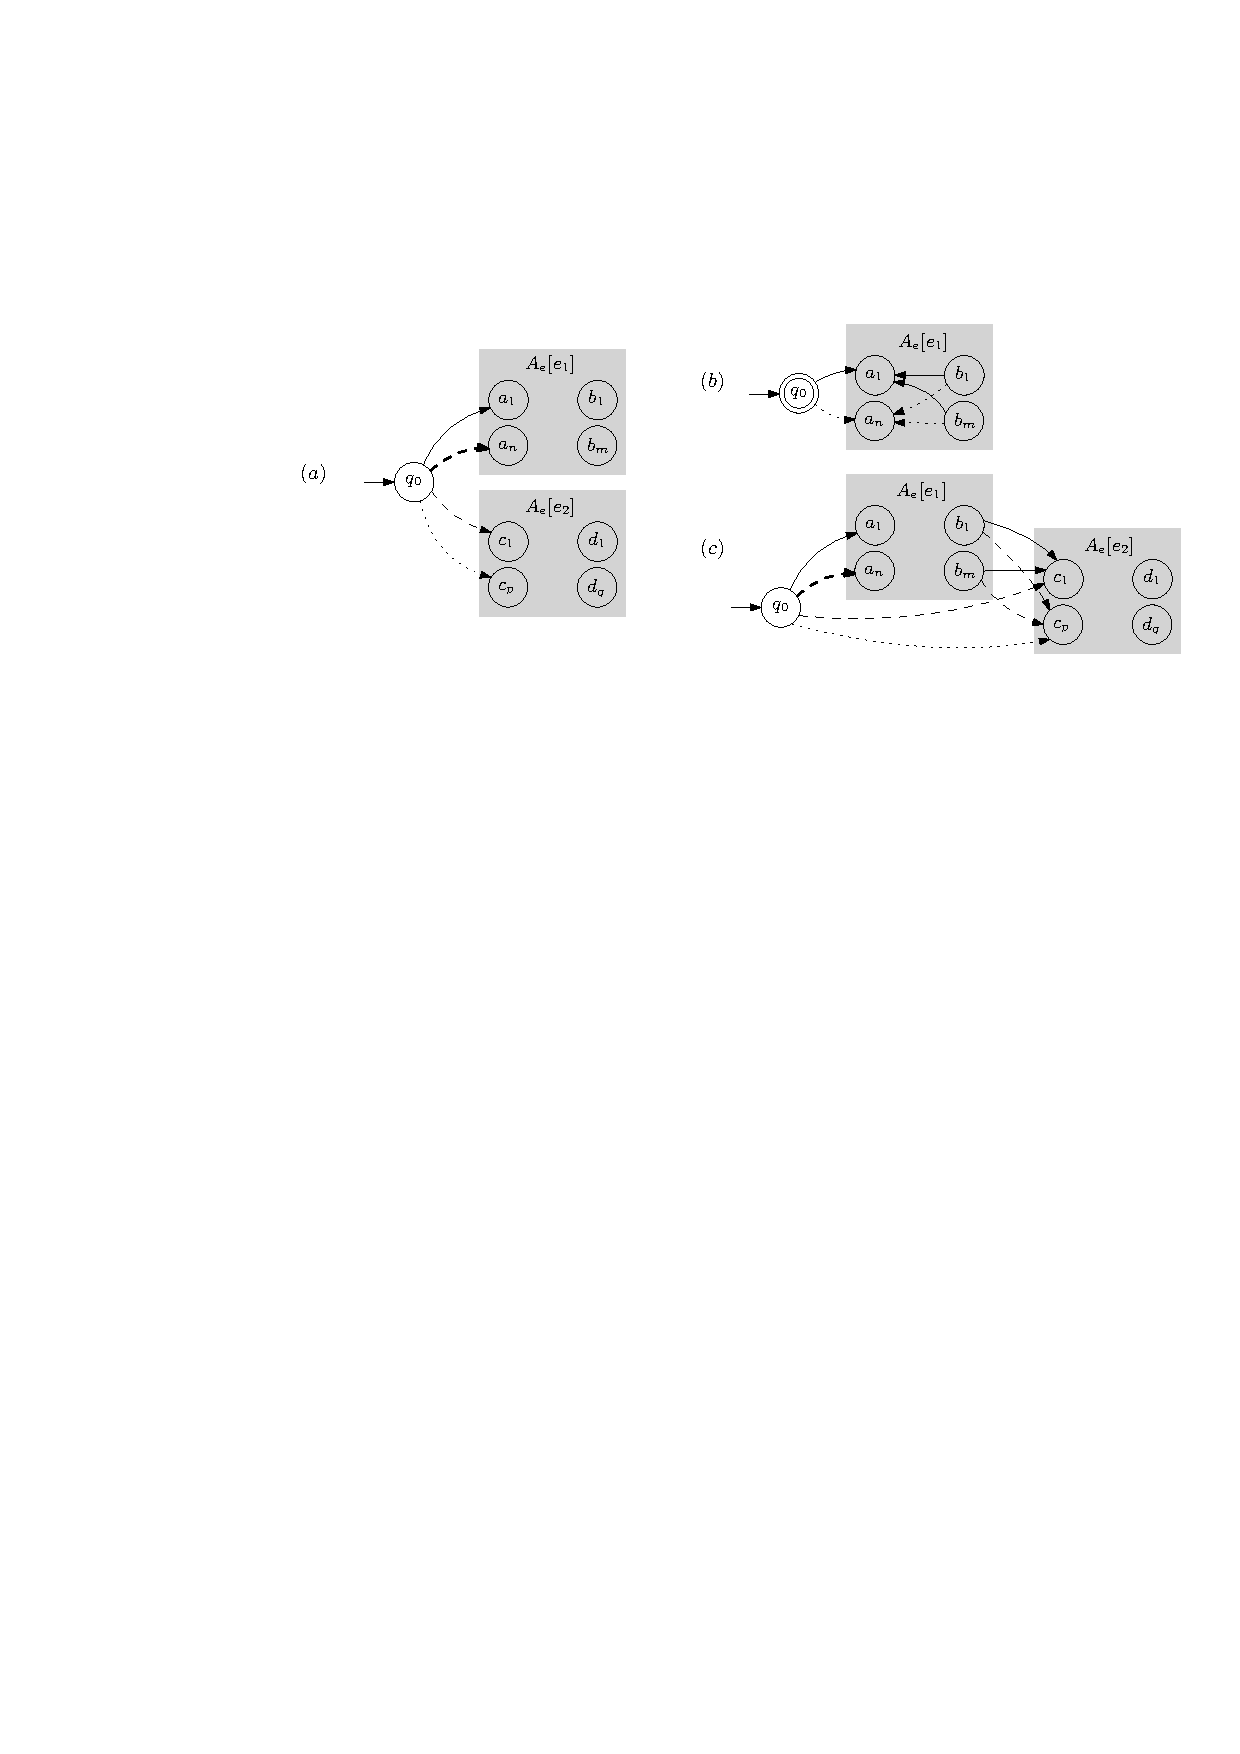
\includegraphics{pglushkov_01}
 \caption{pNFA $A_e$ for (a) $e=e_1+e_2$ (b) $e=e_1^{\ast}$ and (c) $e=e_1 \concat e_2$ where $\varepsilon \in \Lang(e_1)$ and $\varepsilon \notin \Lang(e_2)$. A transition of lower priority is depicted thiner and more densely dotted. }
 \label{fig:pglushkov}
\end{figure*}
 
\subsection{$\replaceall$ with capturing groups and references}

\begin{theorem}[Pre-image of \PSST{}]
  Given a \PSST{} $\psst = (Q_T, \Sigma$, $X, E, \delta_T, q_{0, T}, F_T)$ and \FA{} $A
  = (Q_A, \Sigma, \delta_A, q_{0, A}, F_A)$, we can compute in exponential time an \FA{} $B = (Q_B,
  \Sigma, \delta_B, q_{0, B}, F_B)$ such that $\Lang(B) = \cR^{-1}_T(L)$, where $L$ is the regular language accepted by $A$. 
\end{theorem}
 
\begin{proof}
Intuitively, $B$ simulates the run of $\psst$ on $w$, and records  for each $x \in X$ the set of state pairs $(p, q) \in Q_A \times Q_A$ such that starting from $p$, $A$ can reach $q$ after reading the string represented by $x$. Moreover, $B$ also records all the states accessible from a run with higher priority, and ensure the current run is accepted by $\psst$.

Formally, $Q_B = Q_T \times (\cP(Q_A \times Q_A ))^{X} \times \cP(Q_T)  $, $q_{0, B} = (q_{0, T}, \rho_{\varepsilon}, \emptyset)$ where $\rho_{\varepsilon} (x) = \{(q, q) \mid q \in Q\}$ for each $x \in X$, and $\delta_{B}$ comprises the tuples $((q, \rho, S), a, (q_i, \rho', S'))$ such that there exists $s \in \left((X \cup \Sigma\right)^*)^X$ satisfying
\begin{itemize}
\item $\delta_T (q, a) = (q_1 \ldots q_i \ldots q_m)$, 
\item $s = E(q,a,q_i)$.
\item $S' = \delta_T^{\ast} (S, a) \cup \{ q_1, \ldots, q_{i - 1} \}$, where $\delta_T^{\ast}(S,a) = \{q' \mid \exists q \in S, q' \in \delta_T(q,a)\}$.
\item and $\rho'$ is obtained from $\rho$ and $s$ as follows: for each $x \in X$, if $s(x) = \varepsilon$, then $\rho'(x) = \{(p, p) \mid p \in Q_A\}$, otherwise, let $s(x) = b_1 \cdots b_\ell$ with $b_i \in \Sigma \cup X$ for each $i \in [\ell]$, then $\rho'(x) = \theta_1 \circ \cdots \circ \theta_\ell$, where $\theta_i = \delta^{(b_i)}_A$ if $b_i \in \Sigma$, and $\theta_i = \rho(b_i)$ otherwise.
%
%$\rho'(x) = \theta_\ell$ such that $\theta_0 = \{(p,p) \mid p \in Q_A\}$, and for each $i \in [\ell]$, if $b_i \in \Sigma$, then $\theta_i = \{(p, p') \mid (p, p'') \in \theta_{i-1}, (p'', b_i, p') \in \delta_A \mbox{ for some } p''\}$, otherwise, $\theta_i = \theta_{i-1} \cdot \rho(x)$. 
\end{itemize}

Moreover, $F_B$ is the set of states $(q, \rho, S) \in Q_B$
such that
\begin{enumerate}
  \item $F_T (q)$ is defined,
  \item For any $q' \in S$, $F_T (q')$ is not defined
  
  \item if $F_T(q) = \varepsilon$, then $q_{0, A}  \in F_A$, otherwise, 
let $F_T(q) = b_1 \cdots b_\ell$ with $b_i \in \Sigma \cup X$ for each $i \in [\ell]$, then $(\theta_1 \circ \cdots \circ \theta_\ell) \cap (\{q_{0,A}\} \times F_A) \neq \emptyset$, where for each $i \in [\ell]$, if $b_i \in \Sigma$, then $\theta_i = \delta^{(b_i)}_A$, otherwise, $\theta_i = \rho(b_i)$.
\end{enumerate}
\end{proof}

\begin{remark}
%  The construction above is actually very simple. The automaton N simulates
%  the run of NSST T, together with the \tmtextit{summary} of M when a variable
%  of T in inputed. The construction should be exponential.
%  
  The construction does not utilize the so-called \tmtextit{copyless}
  property in {\cite{AC10,AD11}},
  thus the construction works for general \PSST{}.
\end{remark}

%%%%%%%%%%%%%%%%%%%%%%%%%%%%%%%%%%%%%%%%%%%%%%%%%%
%%%%%%%%%%%%%%%%%%%%%%%%%%%%%%%%%%%%%%%%%%%%%%%%%%
\hide{
\begin{definition}[Two way NSST?]
  The definition of 2NSST is just like 2FT, allowing bidirectional move of
  NSST's head.
\end{definition}

\begin{note}
  One thing is worth noting about this idea of 2NSST: \tmtextit{the pre-image
  of 2NSST is still computable}. We just use a 2FA N to simulate the 2NSST, in
  the same manner of the construction above. We can then transform the 2FA
  into a one-way FA in exponential time.
  
  However, the expressive power of 2NSST is unknown (yet). I highly suspect
  that 2NSST is equivalent to NSST, since the bidirectional move of head
  provides the same function as variables, to some extent. Anyway, the
  expressive power of NSST should be sufficient now.
\end{note}

All the function expressible by 2FT is also expressible by NSST, like
\tmtextit{split}. Below is an example of what more NSST can express.
}
%%%%%%%%%%%%%%%%%%%%%%%%%%%%%%%%%%%%%%%%%%%%%%%%%%
%%%%%%%%%%%%%%%%%%%%%%%%%%%%%%%%%%%%%%%%%%%%%%%%%%

%\begin{definition}[Regular Expression with capturing group, regex]
%  Suppose $\Gamma$ is some set of variables, x is an element of $\Gamma$. a is
%  a character in $\Sigma$
%  \[ \alpha \colons = \varepsilon |a| \alpha + \alpha | \alpha \circ \alpha |
%     \alpha^{\ast} | (\alpha) \%x \]
%  WLOG, we assume a variable occurs at most once in a regex.
  
%  the semantics of regex is defined as tuple $(w, w_x, w_y, \ldots)$ where w
%  is the whole string matched, and $w_x$ is the string matched by the
%  capturing group marked by x, etc. A more formal definition involves match
%  trees and recursive definition.
%  See{\cite{CSY03,CN09}}
%\end{definition}

\begin{definition}[Semantics of $\replaceall_{e_1, e_2}$]
  Consider the constriant $y = \replaceall_{e_1, e_2}(x)$, where $e_1 \in \regexp[\sf CG]$ and $e_2 \in \refexp$.
  
The semantics of $\replaceall_{e_1, e_2}$ is  similar to that in {\cite{CCH+18}}, where the leftmost and longest matching of
  $e_1$ in $x$ is considered, with the difference that here the replacement string is obtained from a matching of $e_1$ by replacing every reference $\$ n$ in $e_2$ with the string matched by the subexpression corresponding to the $n$-th capturing group.
%  
\zhilin{A more formal definition should be added in the future.}
\end{definition}

\begin{remark}
  In the aforementioned definition of the semantics of $\replaceall_{e_1,e_2}(x)$, the matching of $e_1$ in $x$ is deterministic since the leftmost and longest matching is considered, and the process of matching the subexpressions is captured by the semantics in \ref{regex_semantics}.
  
Therefore, the $\replaceall_{e_1,e_2}(x)$ function can be seen as a precise modeling of that used in practical programming languages, e.g. Javascript. \zhilei{might need exemplification}
\end{remark}


\begin{theorem}
  For each $e_1 \in \regexp[\sf CG]$ and $e_2 \in \refexp$, $\replaceall_{e_1, e_2}$ can be modeled by a $\PSST${} $T_{e_1,e_2}$.
\end{theorem}

\begin{proof}

Suppose pNFA $A_{e_1} =(Q, \Sigma,  \delta, q_0, F)$ is the Glushkov automaton constructed from $e_1 \in \regexp[\sf CG]$ by the modified algorithm in \ref{pNFA_cons}. From the algorithm, we know that $Q$ is the union of the initial state $q_0$ and the set of $a_i$'s where the $i$-th character occurring in $e$ is $a$.

For each subexpression $e'$ of $e_1$, we use $C_{e'}$ to denote the set of subexpressions of $e'$ corresponding to a capturing group in $e'$, i.e. the set $\{v \in S(e')\mid \exists v'. v=(v')\}$.

For each state $a_i$ of $A_{e_1}$, we define $C(a_i)$  as the set $\{ e' \in C_{e_1} \mid a_i \mbox{ is a vertex in }
A_{e_1}[e']\}$. Intuitively, $C(a_i)$ represents the set of subexpressions in $C_{e_1}$ whose values should be updated when entering the state $a_i$ in $A_{e_1}$. 

Moreover, for each $e' \in C_{e_1}$, we use $\ssym(e')$ (resp. $\esym(e')$) to denote the set of marked symbols that can be matched to the first  (resp. last) symbol of a string in $\Lang(e')$. For instance, let $e' = a(ab)^*$, then $\ssym(e') = \{a_1\}$ and $\esym(e') = \{a_1, b_3\}$. 

For each $e' \in C_{e_1}$, we introduce a string variable $x_{e'}$. Besides, a special string variable $x_{res}$ is introduced to store, accumulate, and denote the result of $\replaceall_{e_1,e_2}$. Let $X$ denote the set of these string variables.


Then we construct the \PSST{} $T_{e_1,e_2} = (Q', \Sigma, X, E, \delta', q_0', F')$, by using the idea of parsing automata in \cite{CCH+18}. Note in the below, we omit the priority of some transitions and simply write $q' \in \delta'(q,a)$ instead of $\delta'(q,a)=(q_1,q_2,\ldots,q_n)$. In this case, the priority is immaterial and any combination will work.

At first, $q'_0= (\{ q_0
\}, \tmop{left}, \emptyset)$. The set of transition rules $\delta'$ is defined by the following rules.

\begin{itemize}
  
  \item Suppose $(\rho \{ q_0 \}, \tmop{left}, S) \in Q'$, $a \in \Sigma$,
  $\delta (S, a) \cap F = \emptyset$ and $\delta^{\ast} (\rho \{ q_0 \}, a) \cap F =
  \emptyset$, then
  \[ (\tmop{red} (\delta^{\ast} (\rho \{ q_0 \}, a)) \{ q_0 \}, \tmop{left}, \delta
     (S, a)) \in \delta' ((\rho \{ q_0 \}, \tmop{left}, S), a) \]
  and the corresponding assignment is defined as $s(x_{res}) = res \concat a$ and $s(x_{e'})=x_{e'}$ for
  every $e' \in C_{e_1}$.
  
  \item Suppose $(\rho \{ q_0 \}, \tmop{left}, S) \in Q'$ and $a \in \Sigma$.
  If $\delta (S, a) \cap F = \emptyset$, $\delta^{\ast} (\rho, a) \cap F = \emptyset$
  and $\delta (q_0, a) \nsubseteq \delta (S, a) \cup \delta^{\ast} (\rho, a)$, then
  for every $q' \in \delta (q_0, a) \backslash \delta (S, a) \cup \delta^{\ast}
  (\rho, a)$, we have
  \[ (\{ q' \}, \tmop{long}, \delta (S, a) \cup \delta^{\ast} (\rho, a)) \in \delta'
     ((\rho \{ q_0 \}, \tmop{left}, S), a) \]
  and $s$ is the assignment function defined as follows: $s(x_{e'}) = a$ for every $e'  \in C(q')$, and $s(y)=y$ for every other string variable $y \in X$.
  
  \item Suppose $(\{ q \}, \tmop{long}, S) \in Q',$ and $a \in \Sigma$. If
  $\delta (S, a) \cap F = \emptyset$, $\delta (q, a) \nsubseteq \delta (S,
  a)$, and $\delta (q, a) \backslash \delta (S, a) = \{ q_1, \ldots,
  q_n \}$, where $\delta (q, a) = \ldots q_i \ldots q_j \ldots$ for all $i < j$,
  we have $\forall i \in [n]$
  \[ (\{ q_i \}, \tmop{long}, \delta (S, a)) \in \delta' ((\{ q \},
     \tmop{long}, S), a) \]
  and the transition to $(\{ q_i \}, \tmop{long}, \delta (S, a))$ is more prioritized than the transition to
  $(\{ q_j \}, \tmop{long}, \delta (S, a))$ for all $i < j$. 
  
  For any $i \in [n]$, the corresponding assignment $s_i$ is defined as follows:
  
  Suppose $\Theta = \{e' \mid e' = e''^*  \wedge
  q \in \esym(e'') \wedge q_i \in \ssym(e'') \}$ and $C_{\Theta}$ denotes the set of subexpression $e''$ such that $e'' \in C_{e'}$ for some $e' \in \Theta$.
Then 
\begin{itemize}
\item for each $e \in C_{\Theta} \cap C(q_i)$, $s(x_e) = a$,
%
\item for each $e \in C_{\Theta} \setminus C(q_i)$, $s(x_e) = \varepsilon$, 
%
\item for each $e \in C(q_i) \setminus C_\Theta$, $s(x_e) = x_e \concat a$,
%
\item for each $e \in X \setminus (C_\Theta \cup C(q_i))$, $s(x_e)= x_e$.
\end{itemize}

    \item Suppose $(\{ q \}, \tmop{long}, S) \in Q'$, and $a \in \Sigma$. If
  $\delta (S, a) \cap F = \emptyset$, and $\delta (q, a) \cap F = \{ q_1,
  \ldots, q_n \}$, where $\delta (q, a) = \ldots q_i \ldots q_j \ldots$ for all
  $i < j$, we have $\forall i \in [n]$,
  \[ (\{ q_0 \}, \tmop{left}, \delta (S, a) \cup \{ q_i \}) \in \delta' ((\{ q
     \}, \tmop{long}, S), a) \]
  and the transition to $(\{ q_0 \}, \tmop{left}, \delta (S, a) \cup \{ q_i \})$ is more
  prioritized than the transition to $(\{ q_0 \}, \tmop{left}, \delta (S, a) \cup \{ q_j \})$
  for all $i < j$.
  
  For every $i \in [n]$, the corresponding assignment $s_i$ is defined as follows:
  
  Suppose $\Theta = \{e' \mid e' = e''^*  \wedge
  q \in \esym(e'') \wedge q_i \in \ssym(e'') \}$ and $C_{\Theta}$ denotes the set of $e''$ such that $e'' \in C_{e'}$ for some $e' \in \Theta$. Then $s (x_{res}) = x_{res}  \concat b_1   \ldots  b_n$ such that $e_2 = a_1 \ldots a_n$, and for each $i \in [n]$, if $a_i  \in \Sigma$, then $b_i = a_i$, otherwise, $a_i = \$ j$ for some $j$, let $e' \in C_{e_1}$ be the subexpression corresponding to the $j$-th capturing group of $e_1$, then:
  
  \begin{itemize}
\item if $e' \in C_{\Theta} \cap C(q_i)$, $b_j = a$,
%
\item if $e' \in C_{\Theta} \setminus C(q_i)$, $b_j = \varepsilon$, 
%
\item if $e' \in C(q_i) \setminus C_\Theta$, $b_j= x_{e'} \concat a$,
%
\item if $e' \in X \setminus (C_\Theta \cup C(q_i))$, $b_j = x_{e'}$.
\end{itemize}
  
  Moreover, $s(y) = \varepsilon$ for every other variable $y \in X$
  
  \item Suppose $(\rho \{ q_0 \}, \tmop{left}, S) \in Q'$, $a \in \Sigma$,
  $\delta (S, a) \cap F = \emptyset, \delta^{\ast} (\rho, a) \cap F = \emptyset,
  \delta (q_0, a) \cap F = \{ q_1, \ldots, q_n \}$ where $\delta (q, a) =
  \ldots q_i \ldots q_j \ldots$ for all $i < j$. We have for every $i \in [n],$
  \[ (\{ q_0 \}, \tmop{left}, \delta (S, a) \cup \delta^{\ast} (\rho, a) \cup \{ q_i
     \}) \in \delta' ((\rho \{ q_0 \}, \tmop{left}, S), a) \]
  and the transition to $(\{ q_0 \}, \tmop{left}, \delta (S, a) \cup \delta^{\ast} (\rho, a) \cup \{
  q_i \})$ is more prioritized than the transition to $(\{ q_0 \}, \tmop{left}, \delta (S, a)
  \cup \delta^{\ast} (\rho, a) \cup \{ q_j \})$ for all $i < j$.
  
  For every $i \in [n]$, the corresponding assignment $s_i$
  is defined as:
  
  $s (x_{res}) = x_{res}  \concat b_1   \ldots  b_n$ such that $e_2 = a_1 \ldots a_n$, and for each $i \in [n]$, if $a_i  \in \Sigma$, then $b_i = a_i$, otherwise, $a_i = \$ j$ for some $j$, let $e' \in C_{e_1}$ be the subexpression corresponding to the $j$-th capturing group of $e_1$, then if $e' \in C(q_i)$, $b_j = a$, otherwise $b_j = \varepsilon$

  Moreover, $s(y) = \varepsilon$ for every other variable $y \in X$
  
\end{itemize}
The output function $F'$ is simple: $F' (q) = x_{res}$  iff $q = (-, \tmop{left}, -) $.
\end{proof}



\section{Implementation}

\section{Experiments}

%% Acknowledgments
\begin{acks}                            %% acks environment is optional
	%% contents suppressed with 'anonymous'
	%% Commands \grantsponsor{<sponsorID>}{<name>}{<url>} and
	%% \grantnum[<url>]{<sponsorID>}{<number>} should be used to
	%% acknowledge financial support and will be used by metadata
	%% extraction tools.
\end{acks}
%% Bibliography
\bibliography{string}

%% Appendix
\appendix
\section{Appendix}

 


\end{document}
